%auto-ignore
\section{Related Work}

\subsection{Internet-NLP}

\subsubsection{NLP Models with Knowledge Base and Retriver}

These approaches are one the two most popular current solution for NLP tasks to be done without context. It utilizes an knowledge base, a retriever for this data and a LM depending on the use case for example (this list is not extensive):

\begin{itemize}[leftmargin=1em]
    \item question answering: LinkBERT or T5 \cite{https://doi.org/10.48550/arxiv.2203.15827, https://doi.org/10.48550/arxiv.1910.10683}
    \item NLI: CrossEncoder models BERT or DeBERTa \cite{thakur-2020-AugSBERT, https://doi.org/10.48550/arxiv.1810.04805, https://doi.org/10.48550/arxiv.2006.03654}
\end{itemize}

This allows for no-context NLP applications (especially question and answering) to function without any context given, due to knowledge base and retriver providing the context. An representation of this is shown in illustration \ref{fig:CurrSolTwoImg} \cite{https://doi.org/10.48550/arxiv.2201.09651}.

\subsection{Internet-NLP's NLP models}

\subsubsection{LinkBERT}

\begin{figure}
    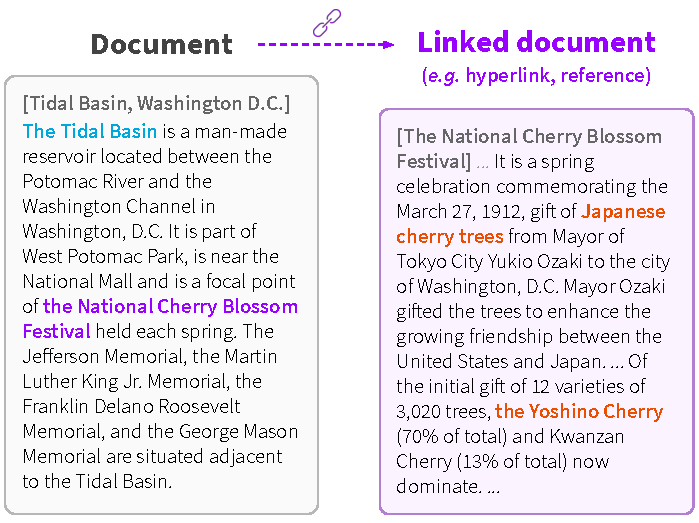
\includegraphics[width=1.0\columnwidth]{fig_motivation_v8.pdf}
    \caption{This is an illustration of example of how LinkBERT utilizes hyperlinks to make a graph corpus \cite{https://doi.org/10.48550/arxiv.2203.15827}.}
    \label{fig:LinkBERTGraphExample}
\end{figure}

\begin{figure}
    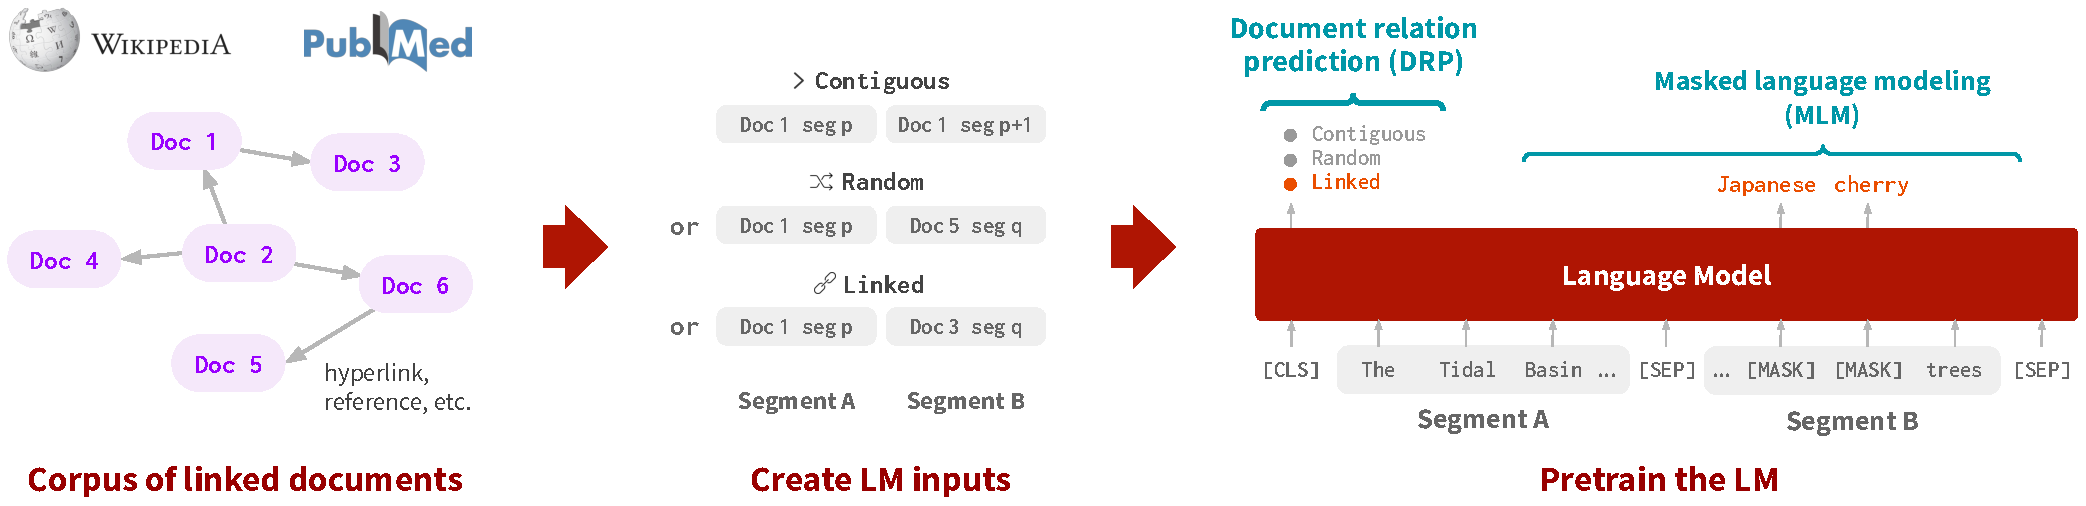
\includegraphics[width=1.0\columnwidth]{fig_overview_v13.pdf}
    \caption{This is an illustration of example of how LinkBERT makes a graph corpus \cite{https://doi.org/10.48550/arxiv.2203.15827}.}
    \label{fig:LinkBERTGraphIllustration}
\end{figure}

LinkBERT is a NLP model that is a pre-trained BERT \cite{https://doi.org/10.48550/arxiv.1810.04805} model that is trained on a graph-based corpus of documents from not only documents but also the hyperlinks in documents. It utilizes a "fusion of graph-based and language-based self-supervised learning" \cite{https://doi.org/10.48550/arxiv.2203.15827}. It gains better performance on graph-based data corpus than other pre-trained NLP models due to it being trained with utilizing graph-based self-supervised learning. 

These are illustrations that explain LinkBERT's graph-based and language-based fusion:

\begin{itemize}[leftmargin=1em]
    \item This illustration shows how hyperlinks can contain crucial information: \ref{fig:LinkBERTGraphExample}.
    \item This illustration shows how LinkBERT \cite{https://doi.org/10.48550/arxiv.2203.15827} makes a graph from links: \ref{fig:LinkBERTGraphIllustration}.
\end{itemize}

For training the Internet-NLP and LM for Text2Text-generation for question answering would be utilizing the fusion of graph-based and language-based learning LinkBERT revolutionized \cite{https://doi.org/10.48550/arxiv.2203.15827}.

\subsection{Internet-NLP's NLI models}

\subsubsection{Cross-Encoder NLI Models}

\begin{figure}
    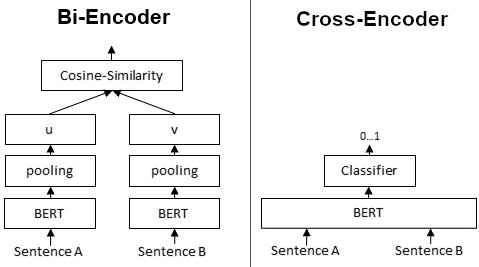
\includegraphics[width=1.0\columnwidth]{Bi_vs_Cross-Encoder.png}
    \caption{This is an illustration of how NLI using Cross-Encoders vs Bi-Encoder work like \cite{thakur-2020-AugSBERT}.}
    \label{fig:CrossEncoderNLI}
\end{figure}

NLI compares two sentences to given an output of entailment (true), neutral or contradiction (false).

Utilizing Cross-Encoder for NLI applications that allow for the utilization of Cross-Encoder (an illustration of Cross-Encoders \ref{fig:CrossEncoderNLI}) where two sentence are passed simultaneously, and then utilizing a classifier to get the output of 0 to 1 which goes from contradiction to entailment \cite{thakur-2020-AugSBERT, https://doi.org/10.48550/arxiv.1908.10084}.
